\setcounter{step}{0}
%------------------------------------------
% information doc
\subsection{Hokaido krémová}
\PrepTime{15}
\CookingTime{10}
\CookingTempe{180}
\TypeCooking{Varenie}
\NbPerson{4}
\Image{0 0 430 430}{images/florentin} %style 2
%------------------------------------------

\begin{ingredient}
%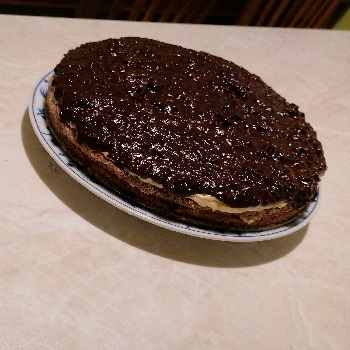
\includegraphics[height=5.5cm]{images/daim}
\def\portions{4}%
\textbf{{\normalsize Ingrediencie (\portions porcie):}}
%\vspace{0.5cm}
\begin{main}
	\item 1 tekvica hokaido
	\item 250ml smotana na varenie
	\item soľ, vegeta
	\item cibuľa
\end{main}
\end{ingredient}
\begin{recipe}
\textbf{{\normalsize Príprava:}}
\begin{enumerate}



\item{Popražíme cibuľu a pridáme umytú nakrájanú tekvicu (aj so šupkou)}
\item{Zalejeme vodou, dochutíme, necháme prevrieť}
\item{Pridáme smotanu, pomixujeme}
\item{Necháme prevrieť}

\end{enumerate}
\end{recipe}

\begin{notes}

\end{notes}	
\clearpage